\documentclass[12pt]{article}
\usepackage[a4paper]{geometry}
\usepackage{blindtext}
\usepackage{titlesec}
\usepackage{amsmath,amssymb}
\usepackage{graphicx}
\usepackage[font=footnotesize]{caption}
\usepackage{subcaption}
\usepackage{dsfont}
\usepackage{xcolor}
\usepackage[numbers,link]{natbib}
\usepackage[colorlinks=true,linkcolor=black,citecolor=red,urlcolor=red]{hyperref}
\usepackage[toc,page]{appendix}
\pagenumbering{gobble}


%%%%%%%%%%%%%%%%%%%%%%%%%%%%%%%%%%%%%%%%%%%%%%%%%%%%%% TITLE %%%%%%%%%%%%%%%%%%%%%%%%%%%%%%%%%%%%%%%%%%%%%%%%%%%%%%
\title{\textbf{Investigation of Quantum Resources in Two--Level Systems Coupled to Quantum Harmonic Oscillators}}
\author{Rowan Adeya}
\date{}
\begin{document}

\maketitle

\newpage

\vspace{\fill}
\begin{abstract}
    Abstract Here.
\end{abstract}
\vspace{\fill}

\newpage
\pagenumbering{arabic}
\tableofcontents

\newpage
%%%%%%%%%%%%%%%%%%%%%%%%%%%%%%%%%%%%%%%%%%%%% INTRODUCTION %%%%%%%%%%%%%%%%%%%%%%%%%%%%%%%%%%%%%%%%%%%%%%%%%%%%%%
\section{Introduction}

Entanglement and coherence are fundamental Quantum Resources which define the behaviour of composite quantum systems. Entanglement is a basis--independent measure of the quantum correlation between subsystems of a
composite system, indicating how much the system’s state deviates from a separable (product) state. It is a uniquely quantum mechanical feature which enables us to utilise non--local correlations, and has had a significant role in advancements of quantum information theory and quantum computation and communication. In contrast, coherence is a basis--dependent measure that describes the ability of a system to remain in a quantum superposition state. We may use coherence to distinguish between quantum and classical regimes, and is often considered as one of the most important features of modern quantum mechanics. However, coherence is fragile and maintaining coherent systems is one of the key challenges in quantum computation [\textbf{Quote x 3}]. \\
\\
One of the simplest composite systems which we may investigate these quantum resources is a Two--Level system (TLS) coupled to a Quantum Harmonic Oscillator (QHO). TLSs naturally manifest in quantum computation as qubits, making qubit–qubit interactions a natural environment for the study of quantum resources. On the other hand, in natural physical systems, we often find TLSs (such as two--level atomic states) coupled to other systems, and more often than not, this is in the form of a QHO. Thus, for these physical systems, it is important to introduce models which convey the type of interactions between the TLS and QHO. 

A canonical and fundamental model is the Jaynes--Cummings Model (JCM). It models a TLS coupled to a single quantised mode of a QHO, representing TLS excitation when a photon is destroyed, and de--excitation when a photon is created. The JCM is often used in the context of circuit QED, cavity QED and other systems such as NV centres [\textbf{Quote}]. The simplicity of the JCM allows for analytical solutions and insights into the dynamics of TLS--QHO systems, but is limited in its ability to capture the richer behaviour found in more complex systems. The Exciton–Vibration model (EVM) is one such extension. It can, for example, describe a dimer (two coupled TLSs) each interacting with its own vibrational mode, modelled as a QHO.\\
\\
Together, these models illustrate the ways in which TLS–QHO interactions arise across a multitude of physical systems, motivating the central question of this work: How do entanglement and coherence manifest in such joint TLS--QHO systems? Understanding this question would deepen our knowledge of quantum resources, and how they can be exploited further in quantum information science and quantum computation. \\
\\
This paper is organised as follows: we begin by discussing the theoretical framework of the Jaynes--Cummings Model, Exciton--Vibration Model and Open Quantum Systems in Section 2. Section 3 explores various measures of entanglement and coherence. Then, we analyse both subsystem populations and the quantum resources in these models via analytical and numerical results in Section 4. Finally, Section 5 presents concluding remarks and possible directions for future research.




























\newpage
%%%%%%%%%%%%%%%%%%%%%%%%%%%%%%%%%%%%%%%%%%%%% TLS--QHO SYS %%%%%%%%%%%%%%%%%%%%%%%%%%%%%%%%%%%%%%%%%%%%%%%%%%%%%%
\section{Two--Level Systems Coupled to Quantum Harmonic Oscillators}

In order to understand how entanglement and coherence manifest in both our models, we must first understand each individual system: the Two--Level System (TLS) and the Quantum Harmonic Oscillator (QHO). Then, we may examine their interactions as a composite quantum system.\\
\\
A TLS is a simple yet fundamental quantum mechanical system which can occupy only two distinct energy states. A state vector describing a TLS may be written as:

\begin{equation}
    |\psi_{\scriptscriptstyle \text{TLS}}\rangle = \alpha|0\rangle + \beta|1\rangle,
\end{equation}

where $|0\rangle$ and $|1\rangle$ are the basis vectors describing the lower and higher energy states respectively, spanning a 2--dimensional Hilbert Space, $\mathcal{H}_{\scriptscriptstyle \text{TLS}}$ , and $\alpha$ and $\beta$ are the complex amplitudes associated with each basis vector. A TLS may be represented by many quantum systems. Most notably, its simplest form is a qubit, which is often used in quantum computation. However, it may also be represented by an atom, with $|0\rangle \rightarrow |g\rangle$ representing the ground (lowest energy) state of an atom, and $|1\rangle \rightarrow |e\rangle$ representing the excited (highest energy) state. Quantum systems may also reduce to an effective TLS if we decide to truncate a system to only two possible energy states. \\
\\
A QHO is another fundamental quantum mechanical model which describes a system with evenly spaced energy levels, and a quantised energy spectrum. A general state vector describing a QHO may be written as:

\begin{equation}
|\psi_{\scriptscriptstyle \text{QHO}}\rangle = \sum_{n=0}^\infty c_n |n\rangle,
\end{equation}

where $|n\rangle$ is the n$^{th}$ Fock state (a state with exactly n quanta of excitation), spanning an infinite--dimensional Hilbert Space $\mathcal{H}_{\scriptscriptstyle \text{QHO}}$, and and $c_n$ are the complex amplitudes associated with each Fock state. A QHO may represent a field confined in a cavity, or a molecular vibration (as we shall see in Sections \ref{JCM_Theory}, \ref{EVM_Theory}).\\
\\
The TLS--QHO composite quantum system is the tensor product of both systems:

\begin{equation}
    |\Psi\rangle = |\psi_{\scriptscriptstyle \text{TLS}}\rangle \otimes |\psi_{\scriptscriptstyle \text{QHO}}\rangle,
\end{equation}

where $|\Psi\rangle$ now resides in the $\mathcal{H}_{\scriptscriptstyle \text{TLS}} \otimes\mathcal{H}_{\scriptscriptstyle \text{QHO}}$ Hilbert space. The Hamiltonian of such a system may be separated into three parts, one for each subsystem (the free Hamiltonians) and one for the interaction of the two systems:

\begin{equation}
    \hat{H} = \hat{H}_{\scriptscriptstyle \text{TLS}} + \hat{H}_{\scriptscriptstyle \text{QHO}} + H_{\scriptscriptstyle \text{I}}.
\end{equation}

Now that we have introduced the TLS–QHO composite system and its Hamiltonian structure, we turn our attention to specific models of interaction: the Jaynes–Cummings Model and the Exciton–Vibration Model. We then examine Open Quantum Dynamics, before analysing the effects of entanglement and coherence on quantum systems.

\subsection{Jaynes--Cummings Model} \label{JCM_Theory}

The Jaynes--Cummings Model (JCM) is a fundamental and canonical model of a TLS--QHO system. It was originally formulated in the context of Quantum Optics in 1963 by Edwin Thompson Jaynes and Fred Cummings \cite{Context1963-JC_Original} and verified experimentally in the context of cavity QED by Herbert Walther in 1985 \cite{Context1993-JC_Verification}. The model itself describes a system where a single TLS is coupled to a single quantised mode of the QHO. The Hamiltonian describing the JCM may be written as:

\begin{equation} \label{JC_H}
    \hat{H_{\scriptscriptstyle \text{JC}}} = \frac{\hbar\omega_a}{2}\hat{\sigma}_z + \hbar\omega_c\left(\hat{a}^\dagger \hat{a} + \frac{1}{2} \right) + g(\hat{a}\hat{\sigma}_{+} + \hat{a}^\dagger\hat{\sigma}_{-}), 
\end{equation} 
with 
\begin{align*}
    \begin{aligned}
        \hat{H}_{\scriptscriptstyle \text{TLS}} &\equiv \frac{\hbar\omega_a}{2}\hat{\sigma}_z \\
        \hat{H}_{\scriptscriptstyle \text{QHO}} &\equiv \hbar\omega_c\left(\hat{a}^\dagger \hat{a} + \frac{1}{2} \right) \\
        \hat{H}_{\scriptscriptstyle \text{I}} &\equiv \hbar g(\hat{\sigma}_{+}\hat{a} +\hat{\sigma}_{-}\hat{a}^\dagger).
    \end{aligned}
\end{align*}

In Equation \eqref{JC_H}, $\omega_a$ is the excitation frequency of the TLS, $\omega_c$ is excitation frequency of the QHO, and $g$ is the coupling strength constant. $\hat{\sigma}_z, \hat{\sigma}_+, \text{and } \hat{\sigma}_-$ are Pauli spin operators of the form $\hat{\sigma}_z = |1\rangle\langle1| - |0\rangle\langle0|, \hat{\sigma}_+ = |1\rangle\langle0|, \text{and } \hat{\sigma}_- = |0\rangle\langle1|$ which act upon the TLS. The operators $\hat{a}, \hat{a}^\dagger$ act solely on the QHO, such that $\hat{a}|n\rangle = \sqrt{n}|n-1\rangle$ acts to lower the state of the QHO, and $\hat{a}^{\dagger}|n\rangle = \sqrt{n+1}|n+1\rangle$ acts to raise the state of the QHO.\\
\\
One of the greatest strengths of the JCM is its simplicity, which enables the model to be exactly solvable. This simplicity, however, is the result of multiple approximations which, in turn, restricts the applicability of the JCM to certain physical systems within certain energy regimes \cite{General2024-JC_overview}. 

The first approximation is the dipole approximation. Here, we consider the QHO to be uniform, such that the interaction Hamiltonian of the JCM can be modelled by a dipole (with energy $\boldsymbol{\hat{d}}$) in a uniform electric field $\boldsymbol{\hat{E}}$, such that:

\begin{equation*}
    \hat{H}_{\scriptscriptstyle \text{I}} \propto \boldsymbol{\hat{d}} \cdot \boldsymbol{\hat{E}}.
\end{equation*}

The second approximation is the single mode approximation. Here, we take the infinite set of quantised modes of the field and discard all except the the mode whose frequency is closest to the transition frequency of the TLS (the resonant mode where $\omega_a = \omega_c$). Thus, the dynamics may be described as a QHO \cite{General2024-JCM_relevance}. In the dipole approximation, the electric field becomes

\begin{equation*}
    \boldsymbol{\hat{E}}  \propto \hat{a} + \hat{a}^\dagger.
\end{equation*}


The third approximation is the TLS approximation. In many quantum systems, such as atoms, there are many discrete energy levels. The JCM, however, only considers the two lowest energy levels of the system, $|0\rangle$ and $|1\rangle$, and all higher energy levels are neglected. The approximation is only valid, however, when the system is weakly driven, such that the higher energy levels are negligible and the system may be described as a TLS. In the dipole approximation, the dipole energy becomes

\begin{equation*}
    \boldsymbol{\hat{d}}  \propto \hat{\sigma}_{-} + \hat{\sigma}_{+}.
\end{equation*}

The last approximation is the Rotating Wave Approximation (RWA). In the full interaction Hamiltonian, the product of the electric field and dipole operator under the RWA becomes

\begin{equation}
    \boldsymbol{\hat{d}} \cdot \boldsymbol{\hat{E}} \propto (\hat{\sigma}_{-} + \hat{\sigma}_{+})(\hat{a} + \hat{a}^\dagger) \approx \hat{\sigma}_{+}\hat{a} +\hat{\sigma}_{-}\hat{a}^\dagger. 
\end{equation}

The RWA neglects the terms $\hat{\sigma}_{-}\hat{a}, \hat{\sigma}_{+}\hat{a}^\dagger$ of the quadratic expansion, which oscillate rapidly. This approximation, however, is only valid when the coupling strength of the interaction $g$ is much less than the characteristic frequencies, $\omega_a$ and $\omega_c$. \\
\\
These approximations, especially the RWA, restrict the JCM to certain physical regimes. Indeed, the JCM primarily concerns itself with systems in the strong--coupling regime \cite{General2024-JCM_relevance}. We now introduce three key conditions for which to uphold this physical regime:
\begin{equation} \label{JCM_condition_g<omega}
    g \ll \omega_a, \omega_c 
\end{equation} 

must be held so that the RWA remains valid. Furthermore, we introduce the cooperativity parameter,

\begin{equation} \label{JCM_condition_cooperativity}
    C = \frac{4g^2}{\gamma\cdot\gamma_{\scriptscriptstyle th}} > 1
\end{equation}

where $\gamma, \gamma_{\scriptscriptstyle th}$ are the decay rates due to spontaneous atomic emission and thermal decay respectively. Finally, we introduce the normalised coupling parameter, 

\begin{equation} \label{JCM_condition_norm_coupling}
    \zeta = C = \frac{4g^2}{\omega_a\cdot\omega_c} < 0.04
\end{equation}, 

with $\zeta \approx \mathcal{O}(1)$ indicating the ultrastrong--coupling regime in which the condition in equation \eqref{JCM_condition_g<omega} is no longer held, and the discarded terms under the RWA approximation are no longer negligible.\\
\\
If we thus remain in valid coupling regimes, the JCM is a fertile model for studying quantum resources in TLS--QHO systems. In fact, there are certain characteristic features captured by the JCM are key to understanding the nature of light--matter interactions it describes. 

One key characteristic of the JCM is Rabi oscillations, which are the coherent, periodic exchanges of excitation between the TLS and QHO. The interaction Hamiltonian in Equation \eqref{JC_H} creates a flip--flop effect, where an excitation in the TLS causes a photon to be destroyed in the QHO, and de--excitation causes a photon to be created. The interaction Hamiltonian clearly shows this periodic exchange of energy via the coupling of the annihilation operator $\hat{a}$ with the atomic excitation operator $\hat{\sigma}_+$, and $\hat{a}^\dagger$ with $\hat{\sigma}_-$.

This operator coupling further leads to the conservation of the excitation number operator, $\hat{N} = \hat{a}^\dagger \hat{a} + \frac{1}{2}(1 + \hat{\sigma}_z)$. The excitation number operator commutes with the Hamiltonian ($[\hat{N}, \hat{H}_{\scriptscriptstyle \text{JC}}] = 0$) and so $\hat{N}$ is conserved. As a consequence, the JCM only allows transitions between states with the same excitation number, such as $|g, n+1\rangle$ and $|e,n\rangle$. For example, states such as

\begin{equation} \label{JCM_general_state}
    |\psi\rangle = \alpha|g,n+1\rangle + \beta|e,n\rangle
\end{equation} 

are allowed, and such states will be explored in section \ref{res_JCM}.\\
\\
It is clear that the JCM's simplicity, arising from the aforementioned approximations, allows it to capture interesting phenomena such as Rabi oscillations.


















\begin{itemize}
    \item Include a diagram of energy regimes.
    \item Write a small para transitioning into Ex-Vib bit
\end{itemize}

# FINISH LATER THURSDAY


\subsection{Exciton--Vibration Model}  \label{EVM_Theory}
\subsection{Open Quantum Dynamics} \label{OQS_Theory}
\begin{itemize}
    \item Talk about what open quantum systems are. 
    \item Mention markovian vs non-markovian approach. 
    \item Go through the Lindblad equation.
    \begin{itemize}
        \item Derivation (brief)
        \item Approximation
    \end{itemize}
    \item Talk about some of the key properties of the time-derivative of density matrix. 
    \item Compare limits - tends to Von Neumann Equation. 
    \item Talk about vectorisation. 
    \item Mention how this is useful for numerical methods - point to appendix. 
    \item Decoherence!!!!!!
\end{itemize}













































%%%%%%%%%%%%%%%%%%%%%%%%%%%%%%%%%%%%%%%%%%%%% Q RESOURCES %%%%%%%%%%%%%%%%%%%%%%%%%%%%%%%%%%%%%%%%%%%%%%%%%%%%%%
\newpage
\section{Quantum Resources}

Quantum resources are fundamental properties of quantum systems which enable us to perform computations and improve a system's efficiency, and are are essential for leveraging the unique advantages of quantum mechanics over classical physics. Two of the most essential resources which we study are entanglement and coherence. In order to inspect how these resources manifest in TLS--QHO systems, we need to be able to understand and quantify them. This section thus focusses on the explanation and quantification of entanglement and coherence, and how they might be used to learn more about our system in question. 

\subsection{Entanglement}

One of the most celebrated quantum resources is entanglement, a unique quantum phenomenon that describes non--classical correlations between subsystems of a composite quantum system. A total state $|\Psi\rangle$ is said to be entangled if it cannot be written as a product state, that is:

\begin{equation}
    |\Psi\rangle \neq |\psi_A\rangle \otimes |\psi_B\rangle,
\end{equation}

where $|\psi_A\rangle, |\psi_B\rangle$ are the pure states of subsystems A and B respectively, and $|\Psi\rangle$ is entangled. If a state \textit{can} be written as a product state, it is considered separable and exhibits only classical correlations. Entangled states, however, exhibit non--local correlations that can violate Bell Inequalities, something which can be demonstrated using, for example, the GHZ game. Entanglement is central to many quantum protocols, such as teleportation, superdense coding and key distribution. 

In physical systems such as the TLS--QHO, entanglement naturally arises as the two systems interact, thus serving as an indicator of of entanglement the correlations between the subsystems. We shall now explore several ways of quantifying entanglment by studying various measures. 

\subsubsection{Von Neumann Entropy}

For a pure state density matrix $\rho_{\scriptscriptstyle \text{AB}}$ \cite{Entanglement1999-Overview_&REE}, the subsystem of A is  found by taking the partial trace over subsystem B, and vice versa, such that $\rho_{\scriptscriptstyle \text{A}} = tr_{\scriptscriptstyle \text{B}}(\rho_{\scriptscriptstyle \text{AB}})$ and $\rho_{\scriptscriptstyle \text{B}} = tr_{\scriptscriptstyle \text{A}}(\rho_{\scriptscriptstyle \text{AB}})$. The von Neumann entropy of the reduced density operators is then given by:

\begin{equation} \label{VNE_original}
    S(\rho_{\scriptscriptstyle \text{AB}}) = -\text{tr}(\rho_{\scriptscriptstyle \text{A}}\ln\rho_{\scriptscriptstyle \text{A}}) = -\text{tr}(\rho_{\scriptscriptstyle \text{B}}\ln\rho_{\scriptscriptstyle \text{B}}).
\end{equation}

We may simplify this further by considering the subsystem density matrices' eigenvalues. If, for example, we are looking at the von Neumann entropy of subsystem A, we first write the subsystem's density matrix as a spectral decomposition:

\begin{equation} \label{VNE_spectral_decomp}
    \rho_{\scriptscriptstyle \text{A}} = \sum_i \lambda_i|\psi_i\rangle\langle\psi_i|, 
\end{equation}

where $\lambda_i$ and $|\psi_i\rangle$ are the eigenvalues and eigenstates of the subsystem density matrix. Since $\rho_{\scriptscriptstyle \text{A}}$ in \eqref{VNE_spectral_decomp} is diagonal,

\begin{equation} \label{VNE_eigenvals}
\text{tr}(\ln\rho_{\scriptscriptstyle \text{A}}) = \sum_i \ln\lambda_i,\text{ and } \text{tr}(\rho_{\scriptscriptstyle \text{A}}) = \sum_i \lambda_i.
\end{equation}

Inserting equations \eqref{VNE_spectral_decomp}, \eqref{VNE_eigenvals} into \eqref{VNE_original} yields a more manageable formulation of the von Neumann entropy:

\begin{equation}
    \mathcal{E} = S(\rho_{\scriptscriptstyle \text{A}}) = S(\rho_{\scriptscriptstyle \text{B}}) = \sum_i \lambda_i\ln\lambda_i,
\end{equation}

where $\mathcal{E}$ is the entanglement of the total system. The von Neumann entropy is a strong and popular candidate when working with pure density matrices. However, the measure fails to distinguish between classical and quantum correlations for mixed states. As we shall see in section \ref{results}, we use the von Neumann entropy for closed system evolution since we always start in pure states. For open quantum systems, however, since pure states become mixed states during evolution, the von Neumann entropy is no longer appropriate. For mixed states, then, we may use Negativity, which applies to both pure and mixed states. 

\subsubsection{Negativity}

Negativity, a simple measure of entanglement, is defined as

\begin{equation} \label{vne_eqn}
    \mathcal{N} = \sum_i |\lambda_i|,
\end{equation}

where $\lambda_i$ are the negative eigenvalues of the partial transpose of the full system density matrix $\rho_{\scriptscriptstyle \text{AB}}$. The partial transpose of a density matrix is computed by transposing one subsystem of the full density matrix, and is written as $\rho_{\scriptscriptstyle \text{AB}}^{T_A}$ or $\rho_{\scriptscriptstyle \text{AB}}^{T_B}$. 

Negativity is a valid measure for both pure and mixed states, making it a powerful tool for quantifying the entanglement of systems undergoing open quantum evolution. Furthermore, it is said to be a LOCC (Local Operations and Classical Communications) montone \cite{Entanglement2009-Definition}, meaning negativity does not increase under LOCC. Due to these two properties, we shall use negativity to analyse the entanglement of our models under open quantum evolution in section \ref{results}. 
\subsubsection{Other Entanglement Measures}
\begin{itemize}
    \item Should I include this section? I would be putting in concurrence and renyi entropy, but since they dont apply to TLS-QHO systems, is it worth it to include?
\end{itemize}
\subsection{Coherence} \label{coh_theory}

Whilst entanglement captures non--classical correlations between subsystems, coherence reflects the superposition properties within individual subsystems, and is another essential quantum resource we must examine to fully understand the dynamics of TLS--QHO systems.

A quantum state $\rho$ is said to be coherent if it has off--diagonal elements in its matrix form. That is,

\begin{equation}
    \rho = \sum_{i,j}\rho|i\rangle\langle j|,
\end{equation}

where $\rho_{ij} \neq 0$ for $i\neq j$ elements. These off--diagonals are coherences, and in particular they make coherence a basis--dependent quantum resource. For example, let us look at the state $|\psi_{\scriptscriptstyle \text{A}}\rangle = \frac{1}{\sqrt{2}}(|0\rangle + |1\rangle)$. As a density matrix, this takes the form:

\begin{equation*}
    \rho_{\scriptscriptstyle \text{A}} = \frac{1}{2}(|0\rangle + |1\rangle)(\langle0| +\langle1|) \rightarrow \frac{1}{2}
    \begin{pmatrix}
        1 & 1 \\
        1 & 1
    \end{pmatrix}.
\end{equation*}

This density matrix is indeed coherent, as seen by the presence of these off--diagonals. If, however, the state were $|\psi_{\scriptscriptstyle \text{B}}\rangle = |0\rangle$, we would have

\begin{equation*}
    \rho_{\scriptscriptstyle \text{B}} = |0\rangle\langle0| \rightarrow 
    \begin{pmatrix}
        1 & 0 \\
        0 & 0
    \end{pmatrix},
\end{equation*}

which has no off--diagonals and is thus incoherent. As we can see, the presence of off--diagonals in $|\rho_{\scriptscriptstyle \text{A}} \rangle$ is a measure of the superposition of the state, a property which is uniquely quantum. The lack of these off--diagonals therefore implies that, in this measurement basis, the state behaves classically. Coherence thus helps us to identify the 'quantumness' of a state in a given basis by looking at the amount of superposition present. As we saw in section \ref{OQS_Theory}, for open quantum systems, the decay of coherence (decoherence) in the system is incredibly important to monitor and minimise,  since it determines the rate at which the system loses its superposition features and begins to behave classically. We shall now explore several ways of quantifying coherence, so that we may use them for studying the manifestation of quantum resources in our TLS--QHO models. 

\subsubsection{Relative Entropy of Coherence}

A general distance-based coherence measure is defined as:

\begin{equation}
    C_{\scriptscriptstyle\text{D}}(\rho) = \inf_{\sigma \in I} D(\rho,\sigma)
\end{equation}

where D is a distance and we take the infimum over the set of incoherent states, and $\sigma$ is a reference state \cite{Coherence2017-Colloquium}. If, similarly to entanglement, we take the distance measure to be the quantum relative entropy, we obtain the relative entropy of coherence, $C_r$. Moreover, it is equal to the distillable coherence. Thus, we obtain:

\begin{equation} \label{rel_ent_coh}
C_r(\rho) = C_d(\rho) = S(\rho_{diag}) - S(\rho)
\end{equation}

where $S$ is the Von Neumann entropy, and $\rho_{diag}$ is the state obtained by removing all off-diagonal elements. In our simulations, we exclusively use the relative entropy of coherence. This choice is motivated by its widespread adoption and its ease of implementation, whilst still faithfully quantifying coherence via the off--diagonals of the state.

\subsubsection{$l_p$ Norm of Coherence}

The $l_p$ norm of coherence is defined as:

\begin{equation}
    C_l(\rho) = \sum_{i\neq j} |\rho_{i,j}|, 
\end{equation}

This measure is particularly intuitive, as it directly reflects the departure of a quantum state from classicality through the off--diagonal elements of a state. In fact, according to \cite{Coherence2014-seed}, the $l_p$ norm satisfies coherence monotonicity criteria which makes it a valid coherence monotone. Alongside the relative entropy of coherence, it constitutes one of the most general and widely accepted coherence measures. By contrast, coherence measures based on other $l_p$ norms, such as the squared Hilbert–Schmidt norm ($l_2$), while similarly based on off--diagonal elements, may fail to satisfy the full set of monotonicity conditions, and hence do not generally define proper coherence monotones.

We shall not, however, be using this measure because it offers no significant advantage over the relative entropy of coherence in our context. Moreover, since the relative entropy already captures the essential coherence behaviour we aim to quantify, introducing additional measures would add redundancy without providing further insight.\\
\\
We have now established the theoretical foundations necessary to study the manifestation of quantum resources in TLS--QHO systems, including two key models, open quantum evolution, and quantifers for both entanglement and coherence. The following section presents our analytical and computational results, highlighting the characteristic features and regimes of both the Jaynes--Cummings and Exciton--Vibration models. 

%%%%%%%%%%%%%%%%%%%%%%%%%%%%%%%%%%%%%%%%%%%%% RESULTS %%%%%%%%%%%%%%%%%%%%%%%%%%%%%%%%%%%%%%%%%%%%%%%%%%%%%%
\newpage
\section{Results} \label{results}

In this section, we present both analytical and numerical results that illustrate how entanglement and coherence emerge and evolve in TLS--QHO systems under both closed and open evolution dynamics.\\
\\
We begin by examining the closed, unitary dynamics of the JCM, combining both analytical and computational methods. This is followed by a numerical simulation of the Jaynes--Cummings model (JCM) under open system dynamics. We then turn to the Exciton--Vibration model (EVM), analysing its behaviour under closed and open evolution computationally. Lastly, we provide comparative analysis of the two models, highlighting the similarities and differences in their population, coherence and entanglement dynamics. \\
\\
Throughout the computational elements of this paper, we use the QuTip library of the Python coding language. QuTip is a highly developed library with extensive functionality that enables the user to model almost any quantum system. It provides nearly all the required functionality for our simulations, and is well suited for models considered in this work. The only functions define manually are those for computing the relative entropy of coherence and negativity functions, which are included in appendix \ref{appendix_code}. All code required to set up the simulations has been structured into a modular Python class, and is available at {should I include a GitHub link here?}.

\subsection{Population, Entanglement and Coherence of the Jaynes--Cummings Model} \label{res_JCM}

The JCM is a simple yet powerful framework for describing TLS--QHO systems. As mentioned in section \ref{JCM_Theory}, its exact solvability stems from its key approximations, making the JCM an ideal starting point for exploring and understanding the dynamics of TLS--QHO systems, and how quantum resources may manifest.\\
\\
We consider both closed and open evolution of the system using the Jaynes--Cummings Hamiltonian in equation \eqref{JC_H}. The closed dynamics allow for both analytical and computational solutions, whilst open dynamics require numerical treatment.\\
\\
For all computational simulations of the JCM, we restrict the model to the strong coupling regime. We consider the characteristic frequencies of our system ($\omega_a, \omega_c$) to be in resonance with one another, i.e. $\omega_a = \omega_c = \omega$. This is a common method to simplify the JCM, and is also employed during our analytical work in the closed evolution study. We set $\omega = 1.0$ and $\hbar = 1$, such that the system is in natural units, and energy in this system is in units of $\omega$. 

To connect our model to experimentally relevant systems, we interpret $\omega$ as being on the scale of meV, which corresponds to THz frequencies, a regime commonly encountered in cavity QED and quantum dot experiments \cite{General2024-JCM_relevance}. As such, the timescales of the system are in the picosecond (ps) range, ensuring that our simulations represent realistic physical regimes.

We choose the coupling strength $g = 0.05$, and our decay rates for spontaneous emission ($\gamma$) and thermal decay ($\gamma_{\scriptscriptstyle th}$) to be $\gamma = \gamma_{\scriptscriptstyle th} = 0.01$, all in units of $\omega$. These values correspond to a cooperativity parameter of $C = 100 > 1$ and a coupling ratio $g = 0.05 \ll \omega$, satisfying the strong coupling condition given in equation \eqref{JCM_condition_cooperativity} and validating the rotating wave approximation (RWA) via equation \eqref{JCM_condition_g<omega}. Moreover, the normalised coupling parameter in equation \eqref{JCM_condition_norm_coupling} is $\zeta = 0.01 < 0.04$, confirming that the system remains outside of the ultrastrong coupling regime.\\
\\
In order to explore how quantum systems evolve, we must define our initial state. For our closed evolution analytical solutions of the JCM, we consider:

\begin{equation} \label{init_JCM_e0}
    |\psi (\text{t}=0)\rangle = |e, 0\rangle,
\end{equation}

where we have relabelled the TLS subsystem so that $|0\rangle \rightarrow|g\rangle$ represents the ground state, and $|1\rangle \rightarrow |e\rangle$ represents the excited state. This initial state appears in several theoretical treatments of the JCM (e.g., \cite{Entanglement2009-REE_VNapplied}), as it isolates a single excitation in the system and allows for analytical solutions due to photon number conservation.

For \textit{all} computational simulations of the JCM, we consider both \eqref{init_JCM_e0} and:

\begin{equation}
    |\psi (\text{t=0})\rangle = \frac{1}{\sqrt{2}}(|e, 0\rangle + |g,0\rangle).
\end{equation}

This system is particularly well-suited for exploring coherence dynamics, as the superposition introduces off-diagonal elements in the TLS subsystem of the initial state.\\
\\
Now that we have set up the relevant parameters and initial states, we begin by examining the closed evolution of the system.

\subsubsection{Closed Evolution}

Our analytical goal for the closed evolution of the JCM is to see whether we can compute both the von Neumann entropy and relative entropy of coherence by solving the Jaynes--Cummings Hamiltonian. We begin by diagonalising the Hamiltonian, so that we can evolve the initial state $|\psi (\text{t}=0)\rangle = |e, 0\rangle$ using the time evolution operator $\hat{U}(t) = e^{-i\hat{H}t/\hbar}$. We then express the time evolved state as a density matrix, and from there we can use equation \eqref{VNE_spectral_decomp} to find the von Neumann entropy, and equation \eqref{rel_ent_coh} to find the relative entropy of coherence.\\
\\
Recall from equation \eqref{JC_H} that the Jaynes--Cummings Hamiltonian is written as follows:
\begin{equation*}
        \hat{H}_{\scriptscriptstyle \text{JC}} = \frac{\hbar\omega_a}{2}\hat{\sigma}_z + \hbar\omega_c\left(\hat{a}^\dagger \hat{a} + \frac{1}{2} \right) + g(\hat{a}\hat{\sigma}_{+} + \hat{a}^\dagger\hat{\sigma}_{-}).
\end{equation*}

A general state of the JCM, due  to the conservation of the excitation number, is written in equation \eqref{JCM_general_state} as

\begin{equation*}
    |\psi\rangle = \alpha|g,n+1\rangle + \beta|e,n\rangle.
\end{equation*}
\\
We now restrict the system to the $n=0$ excitation subspace, which corresponds to the computational basis \small{\{$|g,1\rangle,|e,0\rangle$\}}. This choice is consistent with our initial condition $|e,0\rangle$. The diagonalisation is simplified by working in the matrix form of $\hat{H}_{\scriptscriptstyle \text{JC}}$.\\
\\
\begin{equation*}
    \hat{H}_{\scriptscriptstyle \text{JC}} = 
    \begin{bmatrix}
        \langle g,1|\hat{H}|g,1\rangle & \langle g,1|\hat{H}|e,0\rangle\\
        \langle e,0|\hat{H}|g,1\rangle & \langle e,0|\hat{H}|e,0\rangle
    \end{bmatrix}
\end{equation*}
\\
\begin{equation*}
=
    \begin{bmatrix}
        \large{\frac{3\hbar\omega_c - \hbar\omega_a}{2}} & \small{\hbar g} \\
        \small{\hbar g} & \large{\frac{\hbar\omega_c + \hbar\omega_a}{2}}
    \end{bmatrix}
\end{equation*}
\\
After solving this matrix for the eigenvalues and eigenstates, we retrieve the diagonalised Hamiltonian written in its eigenbasis:

\begin{equation*}
    \hat{H}_{\scriptscriptstyle \text{diag}} = 
    \begin{bmatrix}
        \hbar\omega_c + k & 0 \\
        0 & \hbar\omega_c - k
    \end{bmatrix},
\end{equation*}

where $k = \hbar\sqrt{\frac{\omega_a^2 + \omega_c^2}{4} - \frac{\omega_a\omega_c}{2} + g^2}$. The eigenstates of $\hat{H}_{\scriptscriptstyle \text{diag}}$ are labelled as \{$|\psi_\pm\rangle$\}, and can be expressed as a superposition of our computational basis as follows:

\begin{equation*}
    |\psi_\pm\rangle = \left(1 + \left(\frac{a\pm k}{\hbar g}\right)^2\right)^{-\frac{1}{2}} \cdot\left(|g,1\rangle + \frac{a\pm k}{\hbar g}|e,0\rangle\right),
\end{equation*}

where $a = \hbar\left(\frac{\omega_a - \omega_c}{2}\right)$. Now that we have our diagonalised Hamiltonian, we write it as the unitary evolution operator:

\begin{equation*}
    \hat{U}(t) = e^{-i\hat{H}t/\hbar}
\end{equation*}
\\ 
\begin{equation*}
    = 
    \begin{bmatrix}
        e^{-i(\omega_c + k/\hbar)t} & 0 \\
        0 & e^{-i(\omega_c - k/\hbar)t}
    \end{bmatrix}.
\end{equation*}

We may retrieve the time--evolved state using the relation:
\begin{equation} \label{unitary_evo_eqn}
    |\psi(t)\rangle = \hat{U}(t)|\psi(\text{t}=0)\rangle.
\end{equation}
\\
However, $\hat{U}(t)$ is in the eigenbasis, a different basis to our initial condition. We must therefore perform a basis transformation on our initial condition, such that $P^\dagger|\psi(\text{t} = 0)\rangle = |\psi'(\text{t} = 0)\rangle$, where $P$ is our transformation matrix whose columns are formed of the eigenstates, and $|\psi'(\text{t} = 0)\rangle$ is our initial condition in the eigenbasis. Performing this operation, we get:

\begin{equation*}
    |\psi'(\text{t} = 0)\rangle = 
    \begin{bmatrix}
        \left(1 + \left(\frac{a + k}{\hbar g}\right)^2\right)^{-\frac{1}{2}}\cdot\left(\frac{a + k}{\hbar g}\right) \\
        \left(1 + \left(\frac{a - k}{\hbar g}\right)^2\right)^{-\frac{1}{2}}\cdot\left(\frac{a - k}{\hbar g}\right)
    \end{bmatrix}.
\end{equation*}
\\
Using equation \eqref{unitary_evo_eqn}, we may then write our final time--evolved state in the eigenbasis as:

\begin{equation*}
    |\psi'(\text{t})\rangle = 
    \begin{bmatrix}
        e^{-i(\omega_c + k/\hbar)t}\cdot\left(1 + \left(\frac{a + k}{\hbar g}\right)^2\right)^{-\frac{1}{2}}\cdot\left(\frac{a + k}{\hbar g}\right) \\
        e^{-i(\omega_c - k/\hbar)t}\cdot\left(1 + \left(\frac{a - k}{\hbar g}\right)^2\right)^{-\frac{1}{2}}\cdot\left(\frac{a - k}{\hbar g}\right)
    \end{bmatrix}.
\end{equation*}
\\
As mentioned in section \ref{coh_theory}, coherence is a basis-dependent measure. We are currently in the eigenbasis of the Jaynes--Cummings Hamiltonian; however, we are interested in measuring the coherence in the computational basis, since it corresponds to the physical states of the atom and field and thus reflects an observable superposition between the atom and cavity states. We perform this transformation this time by using the closure relation, such that:

\begin{equation*}
    \mathds{1} = \sum_i|\phi_i\rangle\langle\phi_i| = |g,1\rangle\langle g,1| + |e,0\rangle\langle e,0|
\end{equation*}

\begin{equation*}
    \rightarrow \text{  } \mathds{1}|\psi'(\text{t})\rangle = |\psi(\text{t})\rangle,
\end{equation*}


where $|\psi(\text{t})\rangle$ is now in the computational basis. Of course, we could have chosen to use the basis transformation matrix method again (as we did with our initial state). We decided upon using the identity method instead to develop and strengthen our understanding of the formal methods of quantum theory. 

We know that our time--evolved state will be in some superposition $|\psi(\text{t})\rangle = \alpha(t)|g,1\rangle + \beta(t)|e,0\rangle$, where $\alpha(t),\beta(t)$ are complex coefficients which are found by performing the basis transformation. Our corresponding time--evolved density operator is:

\begin{equation*}
    \rho(t) = |\alpha(t)|^2|g,1\rangle\langle g,1| + |\beta(t)|^2 |e,0\rangle\langle e,0| + \alpha(t)\beta^*(t)|g,1\rangle\langle e,0| + \alpha^*(t)\beta(t)|e,0\rangle\langle g,1|,
\end{equation*}

which is a pure density operator. We are now equipped to calculate both the von Neumann entropy and relative entropy of coherence. We start with the von Neumann entropy, a measure of entanglement, which we recall from equation \eqref{vne_eqn} is written as 

\begin{equation*}
   \mathcal{E} = S(\rho_{\scriptscriptstyle \text{A}}) = \sum_i \lambda_i\ln\lambda_i,
\end{equation*}

where $\lambda_i$ are the eigenvalues of the density matrix $\rho_{\scriptscriptstyle \text{A}}$. Given a pure density matrix, the von Neumann entropy of either of the subsystems yields the entanglement, $\mathcal{E}$ of the total system. In order to find one subsystem of the density matrix, we trace out the other subsystem using the partial trace. This yields:

\begin{equation*}
        \rho_{\scriptscriptstyle \text{TLS}}(t) = |\alpha(t)|^2|g\rangle\langle g| + |\beta(t)|^2 |e\rangle\langle e|,
\end{equation*}

and

\begin{equation*}
        \rho_{\scriptscriptstyle \text{QHO}}(t) = |\alpha(t)|^2|1\rangle\langle 1| + |\beta(t)|^2 |0\rangle\langle 0|.
\end{equation*}
\\
We can already clearly see that both subsystems are diagonal, and both subsystems have the same eigenvalues of $|\alpha(t)|^2,|\beta(t)|^2$, and so the von Neumann entropy of either subsystem will indeed be the same. To simplify our analytical calculations, we apply the resonance condition, $\omega_a = \omega_c = \omega$, a condition used throughout both closed and open computational evolutions of the JCM. This results in the following simplifications of our parameters: $k = \hbar g$ and $a = 0$. Under resonance, the coefficients reduce to:

\begin{equation*}
    |\alpha(t)|^2 = \frac{1}{2} - \frac{1}{2}\cos gt,
\end{equation*}

and 
\begin{equation*}
    |\alpha(t)|^2 = \frac{1}{2} + \frac{1}{2}\cos gt.
\end{equation*}
\\
Let us choose the TLS subsystem, $\rho_{\scriptscriptstyle \text{TLS}}(t)$. Since the coefficients are a function of $\cos(gt)$, we can consider what happens at three points during the curve: $\cos(gt) = 0,1, \text{and} -1$.\\
\\
At $\cos(gt) = 1, |\alpha(t)|^2 =0 \text{ and } |\beta(t)|^2 = 1$. The von Neumann entropy of this subsystem is thus $0$, and so the entanglement $\mathcal{E}=0$.

At $\cos(gt) = -1, |\alpha(t)|^2 = 1 \text{ and } |\beta(t)|^2 = 0$. The von Neumann entropy of this subsystem is thus $0$, and so the entanglement $\mathcal{E}=0$.

At $\cos(gt) = 1, |\alpha(t)|^2 = \frac{1}{2} \text{ and } |\beta(t)|^2 = \frac{1}{2}$. The von Neumann entropy of this subsystem is thus:

\begin{equation*}
    S(\rho_{\scriptscriptstyle \text{TLS}}(t)) = - \frac{1}{2}\ln\frac{1}{2} - \frac{1}{2}\ln\frac{1}{2}
    = \ln2.
\end{equation*}
\\
For closed evolution of the JCM under the initial condition $|\psi(\text{t} = 0)\rangle = |e,0\rangle$, we find that the entanglement $\mathcal{E}(t)$ oscillates at a rate $g$, with values ranging between $0 \text{ and } \ln2 \approx 0.7$. We verify this in our simulation of the JCM:
%\caption{\normal{von Neumann entropy of the JCM under closed unitary evolution, %starting with an initial condition of $|\psi(\text{t} = 0)\rangle = |e,0\rangle$.}}
\begin{figure}[h]
    \centering
    % First row
    \begin{subfigure}{0.45\textwidth}
        \centering
        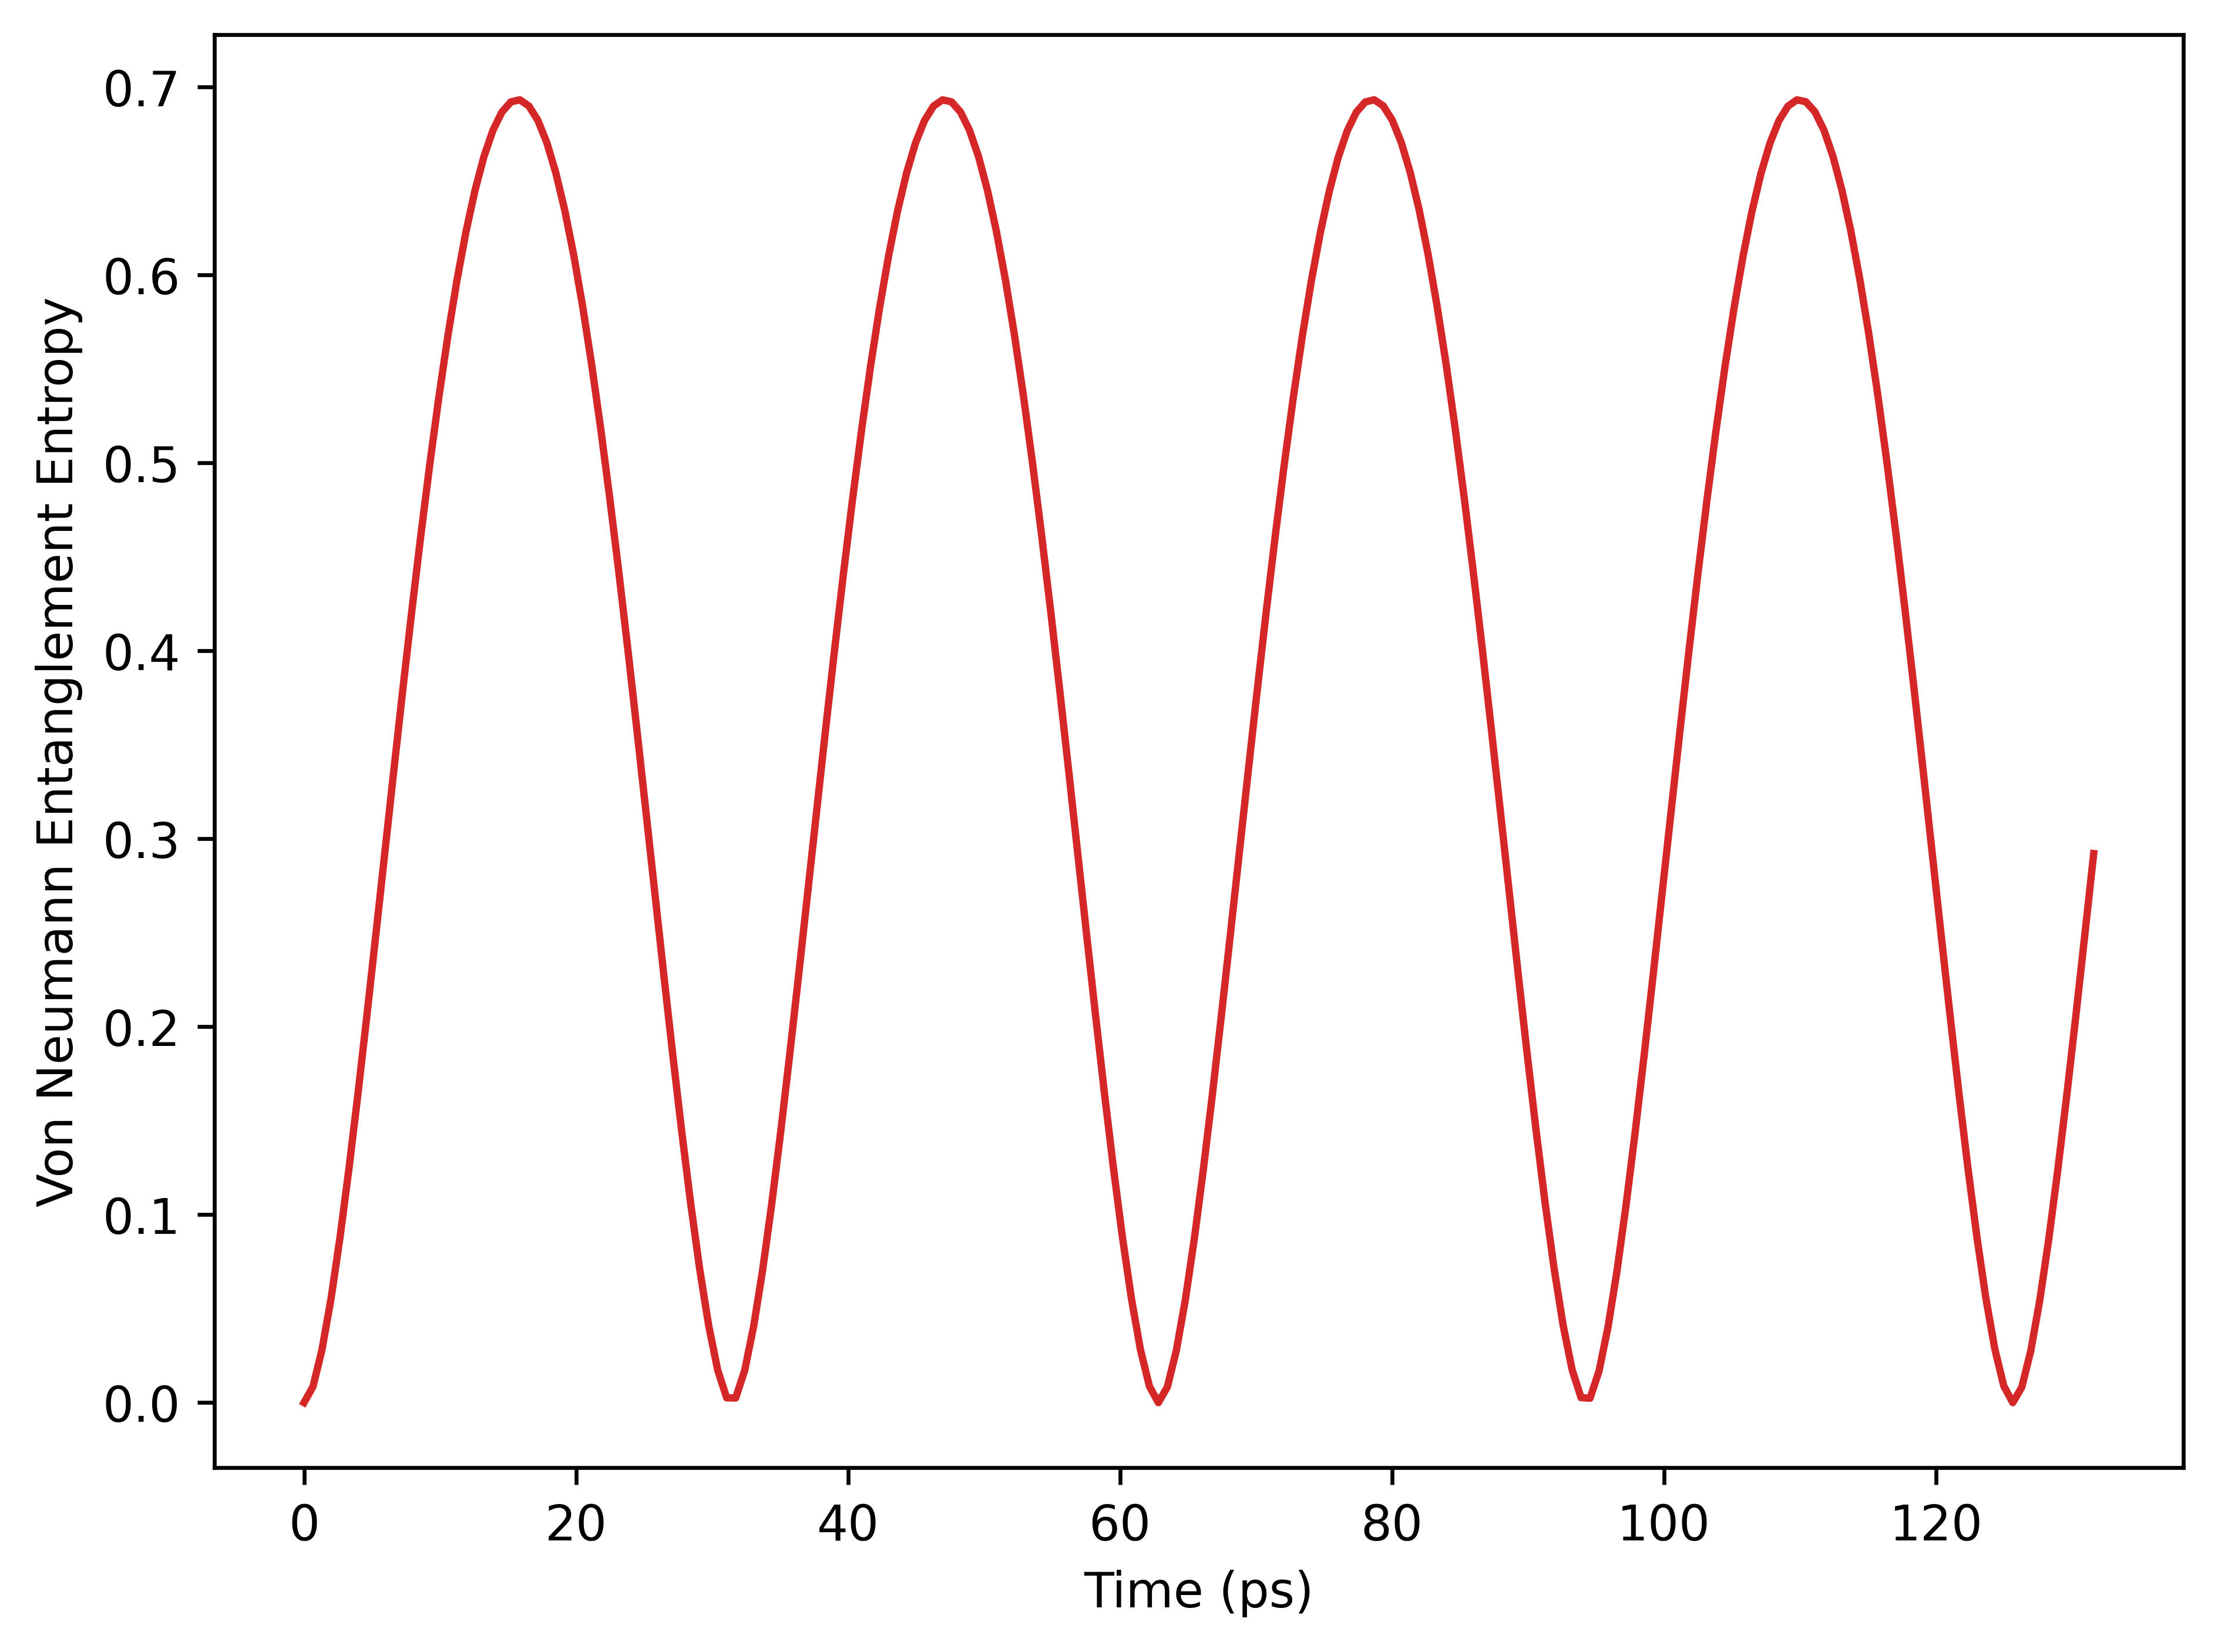
\includegraphics[width=\linewidth]{Research Project/Code/results/JCM/CQS_vne.png}
        \label{fig:JCM_cqs_vne_e0}
    \end{subfigure}
    \begin{subfigure}{0.45\textwidth}
        \centering
        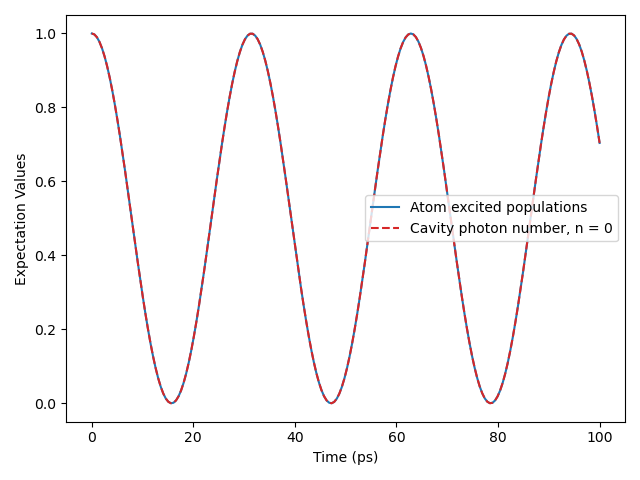
\includegraphics[width=\linewidth]{Research Project/Code/results/JCM/CQS_expt.png}
        \label{JCM_cqs_xpt_e0}
    \end{subfigure}
\end{figure}
In figure \eqref{JCM_CQS_e0_VNE}, we can clearly see the oscillatory pattern of entanglement that we find from our analytical calculations. These oscillations are one of the key features of the JCM: Rabi oscillations. As mentioned in section \ref{JCM_Theory}, the oscillations come from the interaction part of the Hamiltonian:

\begin{equation*}
     \hat{H}_{\scriptscriptstyle \text{I}} = \hbar g(\hat{\sigma}_{+}\hat{a} +\hat{\sigma}_{-}\hat{a}^\dagger),
\end{equation*}

which drives coherent exchange of excitations between the atom and field. The term $\hat{\sigma}_{+}\hat{a}$ describes photon absorption resulting in atomic excitation, whilst $\hat{\sigma}_{-}\hat{a}^\dagger$ corresponds to photon emission with atomic de-excitation. Since $\hat{H}_{\scriptscriptstyle\text{I}}$ commutes with the total excitation number operator, $\hat{N} = \hat{a}^\dagger \hat{a} + \frac{1}{2}(1 + \hat{\sigma}_z)$, evolution is confined to subspaces of fixed $\hat{N}$. So, for the initial state $|e,0\rangle$ where $\hat{N} = 1$, the dynamics occur entirely within the space \small{\{$|g,1\rangle,|e,0\rangle$\}}, producing Rabi oscillations at frequency g. This periodic transfer causes modulation in the entanglement, between  0 (pure states) and $\ln2$ (maximal entanglement for a TLS), as seen in figure~\ref{JCM_CQS_e0_VNE}.\\
\\
We 






\begin{figure}[h]
    \centering
    % First row
    \begin{subfigure}{0.45\textwidth}
        \centering
        \includegraphics[width=\linewidth]{image1.png}
        \caption{First image}
        \label{fig:image1}
    \end{subfigure}
    \hfill
    \begin{subfigure}{0.45\textwidth}
        \centering
        \includegraphics[width=\linewidth]{image2.png}
        \caption{Second image}
        \label{fig:image2}
    \end{subfigure}
    
    \vspace{0.5cm} % Space between rows
    
    % Second row
    \begin{subfigure}{0.45\textwidth}
        \centering
        \includegraphics[width=\linewidth]{image3.png}
        \caption{Third image}
        \label{fig:image3}
    \end{subfigure}
    \hfill

    
    \caption{A $2\times 2$ grid of images.}
    \label{fig:2x2grid}
\end{figure}





















\newpage
\begin{itemize}
    
    \begin{itemize}
        \item Go through the theory completely. 
        \item Explain your expectations.
        \item Go through the code numerically and show some graphs where necessary. 
        \item Explain your results numerical and whether they match expectations. 
    \end{itemize}
\end{itemize}
\subsubsection{Open Evolution}
\begin{itemize}
    \item Mention that you've done only one part analytically, and numerically to verify your results.
    \item For each analytical final result:
    \begin{itemize}
        \item Go through the theory completely. 
        \item Explain your expectations.
        \item Go through the code numerically and show graphs. 
        \item Explain your results numerical and whether they match expectations. 
    \end{itemize}
\end{itemize}
\subsection{Population, Entanglement and Coherence of the Exciton--Vibration Model}
\subsubsection{Closed Evolution}
\subsubsection{Open Evolution}
\subsection{Discussion}




































%%%%%%%%%%%%%%%%%%%%%%%%%%%%%%%%%%%%%%%%%%%%% CONCLUSION %%%%%%%%%%%%%%%%%%%%%%%%%%%%%%%%%%%%%%%%%%%%%%%%%%%%%%
\newpage
\section{Conclusion and Outlook}











































%%%%%%%%%%%%%%%%%%%%%%%%%%%%%%%%%%%%%%%%%%%%% Appendices %%%%%%%%%%%%%%%%%%%%%%%%%%%%%%%%%%%%%%%%%%%%%%%%%%%%%%
\begin{appendices}
    \section{Code Stuff} \label{appendix_code}
\end{appendices}
\newpage

\bibliographystyle{unsrt} 
\bibliography{References/references.bib} 

\end{document}